\documentclass[a4paper]{article}
\usepackage[utf8]{inputenc}
\usepackage{amsmath}
\usepackage{siunitx}
\usepackage[ngerman]{babel}
\usepackage{pgfplots}
\usepackage{hyperref}
\usepackage{pgfplotstable}
\usepackage{csvsimple}

\pgfplotsset{compat=1.15}

\title{GPET\\ Auswertung Versuch 1}

\author{Jonas Otto\\ \href{mailto:jonas@jonasotto.com}{jonas@jonasotto.com} 
   \and Luca Krüger \\ \href{mailto:luca.krueger@uni-ulm.de}{luca.krueger@uni-ulm.de} }
\date{\today}

\begin{document}

\maketitle

\section{Vorbereitung}
    \paragraph{1.}
    Die Kirchhoffschen Regeln beschreiben die Maschen- und Knotenregeln. Die Maschenregel besagt dass die Summe aller Spannungen in einer Masche $0$ ergibt. Die Knotenregel besagt dass die Summe aller Ströme, die in einen Knoten hinein und aus einem Knoten heraus fließen gleich $0$ ist.
    
    \paragraph{2.}
    Der zu messende Strom fließt in den Knoten und danach durch den Shuntwiderstand und den Innenwiderstand des Messgerätes ab. Der Strom wird nach dem ohmschen Gesetz aufgeteilt:
    \begin{eqnarray*}
        \text{Eingangsstrom: }& I_n=n\cdot I_{max}\\
        \text{Strom durch Shunt: }& I_p=n\cdot I_{max}-I_{max} = (n-1) \cdot I_{max}\\
    \end{eqnarray*}
    
    Stromteiler ergibt:
    \begin{eqnarray*}
            &I_{max}&=n\cdot I_{max} \cdot \frac{R_p}{R_i+R_p}\\
        \iff& 1&=n \cdot \frac{R_p}{R_i+R_p}\\
        \iff& R_i+R_p&=n \cdot {R_p}\\
        \iff& R_i&=(n-1) \cdot {R_p}\\
        \iff& R_p&=\frac{R_i}{n-1}\\
    \end{eqnarray*}
    
    \paragraph{3.}
    Der Widerstand berechnet sich wie in 2. : $ R_p=\frac{R_i}{n-1} = \frac{18\si{\ohm}}{9-1} = 2\si{\ohm}$. Gegebenenfalls sollte der Widerstand kleiner gewählt werden, um das Messgerät nicht zu beschädigen, wenn der zu messende Strom größer ist.
    
    \paragraph{4.}
    Bei der maximalen Spannung von $U_B=30\si{V}$ fließt durch den Widerstand ein Strom von $I=\frac{U}{R}=\frac{30\si{V}}{220\si{k\ohm}}=0.14\si{mA}$. Die Leistung beträgt dabei $P=U\cdot I=4.1\si{mW}$, was unterhalb der Spezifikation von $0.125\si{W}$ liegt. Der Spannungsbereich muss also nicht eingeschränkt werden.
    
    \paragraph{5.}
    Die Zeitkonstante des RC Glied beträgt $\tau=R\cdot C$.
    
    \paragraph{6.}
    Nach $\tau$ Sekunden erreicht die Spannung ca $63\%$ der Endspannung. Die Zeitkonstante beträgt also ca $\tau=2.5\si{s}$.
    
    \paragraph{7.}
    Das Verhältnis $\frac{R_0}{R}$ muss $\frac{1}{9}$ sein, das Verhältnis der Kondensatoren $\frac{C_0}{C}$ invers dazu, also $\frac{9}{1}$ sein, sodass die Zeitkonstanten gleich sind und Teilungsfehler behoben werden.

\section{Versuchsauswertung}
    \subsection{Auslesen von Messwerten mit Python}
    %from praktikum import *
    %var_rm = resourceManager()
    %var_instrlist = instr find(var_rm)
    %var_instr = connect Instrument(var_rm, "ASRL6::INSTR")
    %var_read = query cmd(var instr,"READ?")
    %close Instrument(var_instr)
    %close ResourceManager(var_rm)
    
    Der Strom wurde mit den Python-Befehlen aus der Aufgabenstellung erfolgreich über den PC ausgelesen. Die gefundene Gerätenummer lautet ASRL4::INSTR.
 
    \subsection{Widerstandskennlinie}
    
    Für den Versuchsaufbau wird ein $220\si{k\ohm}$ Widerstand in Reihe zum Multimeter an die Spannungsversorgung angeschlossen.
    Im folgenden wurden unterschiedliche Spannungen eingestellt und dazu der Strom durch den Widerstand gemessen.
    Das Messgerät hat laut Spezifikation einen relativen Fehler von $1\%$. Der absolute Fehler des Messgerätes ist sehr gering, weshalb in den Messergebnissen vor allem der relative Fehler eine Rolle spielt.(Beispiel: bei dem kleinsten Messwert von $26,9\si{\micro A}$ liegt der Anteil eines absoluten Fehlers von $2$ counts bei $0,07\%$) Dadurch ist die Widerstandsmessung am genauesten($1,4\%$) wenn der gemessene Strom klein ist.\\
    Im Allgemeinen überwiegt bei höheren Messwerten der relative Fehler und bei sehr kleinen Messwerten der absolute Fehler.\\
    Dass der gemessene Fehler höher ist, als in den Spezifikationen des Messgerätes angegeben liegt unter anderem daran, dass der Widerstand auch eine gewisse Toleranz aufweist.\\
    Der Verlauf der Kennlinie ist proportional. Die Abweichung der Messkurve wird aufgrund des relativen Fehlers des Messgerätes(s.o.) im Verlauf größer.
  
    \begin{center}
    \csvreader[tabular= c c c c c,
    table head={U[\si{V}] & I [\si{\micro A}] & $R [\si{k\ohm}]$ & $\Delta R[\si{k\ohm}]$ & $\rho_R[\%]$\\\hline},
    late after line=\\, /csv/separator=semicolon]%
    {kennlinie.csv}{U=\spannung,I=\i,R(kOhm)=\r,abs=\ea,rel=\er}%
    {\tablenum{\spannung} & \tablenum{\i} & \tablenum{\r} & \tablenum{\ea} & \tablenum{\er}}%
    \end{center}
    
    \begin{center}
    \begin{tikzpicture}
    \begin{axis}[
        title={Widerstandskennlinie},
        xlabel={U [\si{V}]},
        ylabel={I [\si{\micro A}]},
        xmin=0, xmax=30,
        ymin=0, ymax=150,
        xtick={0,10, 20, 30},
        ytick={0, 20, 40, 60, 80, 100, 120, 140},
        legend pos=north west,
        ymajorgrids=true,
        grid style=dashed,
    ]
    %6V 26,9µA
    %12V 53,42µA
    %18V 80,1µA
    %24V 106,9µA
    %30V 133,5µA
     
    \addplot[
        color=blue,
        mark=square,
        ]
        coordinates {
        (0,0)(6,26.9)(12,53.42)(18,80.1)(24,106.9)(30,133.5)
        };
    \addplot[
        color=red,
        domain=0:30,
        ]
        {x/0.220};
    \legend{$I_R$ (Gemessen), $I_R$ (Berechnet)}
    \end{axis}
    \end{tikzpicture}
    \end{center}
    \subsection{Oszilloskop}
    
    Der Funktionsgenerator wird auf eine Sinusschwingung mit Peak-Peak Spannung von 1V eingestellt, Frequenz 1kHz. Der Ausgang wurde mit einem BNC-Kabel mit Kanal 1 des Oszilloskops verbunden. Sowohl durch Ablesen der Zeit als auch durch die Measure Funktion bestätigt sich die Frequenz von 1kHz. Die Measure Funktion zeigt für $V_{pp}$ einen Wert von $1,05 \si{V}$ an.
    Die Ausgangseinstellung des Funktionsgenerators wird auf \glqq Hoch-Z\grqq gestellt, da das Oszilloskop einen hochohmigen Eingang besitzt. Beim Ändern der Einstellung auf eine Ausgangslast von 50\si{\ohm} konnte keine Veränderung beobachtet werden.
    Beim Ändern der Frequenz oder Amplitude musste die Zeit- und Spannungsskala des Oszilloskop entsprechend angepasst werden.
    Beim verschieben des Trigger-Levels verschiebt sich zunächst der Graph nach links oder rechts, sodass der Schnittpunkt des Triggers mit dem Signal in der vertikalen Mittelachse des Bildschirms bleibt. Wenn der Trigger-Level über dem größten Messwert liegt, dann kann der Trigger nicht mehr ausgelöst und das Signal nicht synchronisiert werden.
    
    \subsection{DC- und AC-Einstellungen der Eingänge}
    \paragraph{1}
    Mit dem Funktionsgenerator wurde ein Signal mit $f=10\si{kHz}, V_{pp}=1\si{V}$ und einem DC-Offset von $1\si{V}$ erzeugt und am Kanal 1 gemessen. Das DC-Offset ist am Bildschirm sichtbar, wenn der Eingang auf DC-Kopplung eingestellt ist. Das Offset verschwindet, wenn der Eingang auf AC eingestellt wird. Intern wird bei dem Oszilloskop in dieser Konfiguration ein Kondensator in Reihe mit dem Signal geschlossen, sodass der Gleichanteil in dem Signal verschwindet.
    
    \paragraph{2}
    Als Frequenz der Rechteckschwingung wurde $f=50\si{Hz}$ eingestellt, die Amplitude beträgt $2\si{V}$. Das Oszilloskop ist auf Kanal 1 auf AC eingestellt, das Trigger-Level auf $1\si{V}$. Die Rechteckspannung wird verzerrt dargestellt (Abbildung \ref{fig:rechteckAC}). Die Messung ergibt nun eine Peak-Peak Spannung von $2.67\si{V}$. Dieses Verhalten erklären wir uns damit, dass die Koppelkondensatoren wie ein Hochpass wirken, in dem Zeitabschnitt, in dem das Rechtecksignal konstant ist, geht die gemessene Spannung gegen $0\si{V}$. Dies bestätigt sich auch bei Messungen mit kleinerer Frequenz. In Abbildung \ref{fig:rechteckDC}
    zum Vergleich die Rechteckspannung im DC Modus.
    \begin{figure}
    \caption{Rechteckspannung mit AC Kupplung}
    \centering
    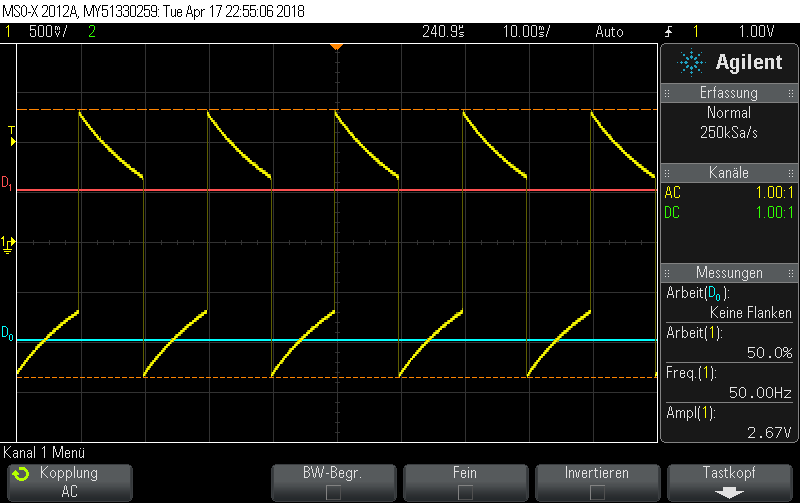
\includegraphics[width=0.7\textwidth]{rechteckAC}
    \label{fig:rechteckAC}
    \end{figure}
    \begin{figure}
    \caption{Rechteckspannung mit DC Kupplung}
    \centering
    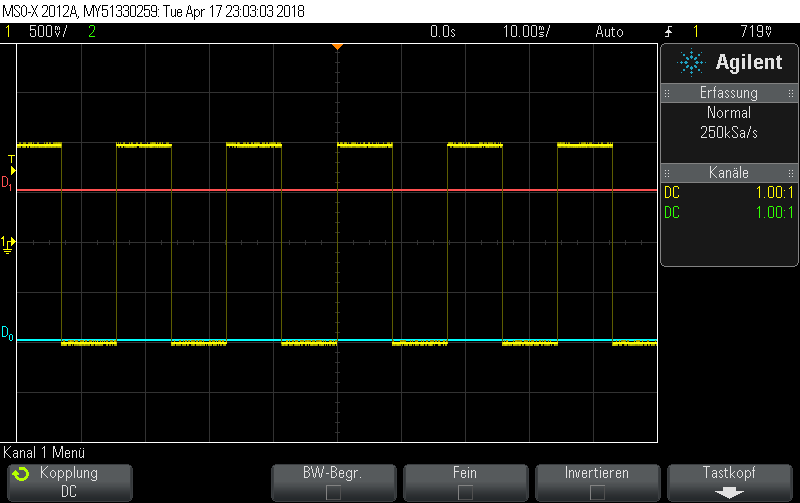
\includegraphics[width=0.7\textwidth]{rechteckDC}
    \label{fig:rechteckDC}
    \end{figure}
    
    \subsection{Kondensator}
    \begin{figure}
    \caption{Manuelle Messung der Anstiegszeit}
    \centering
    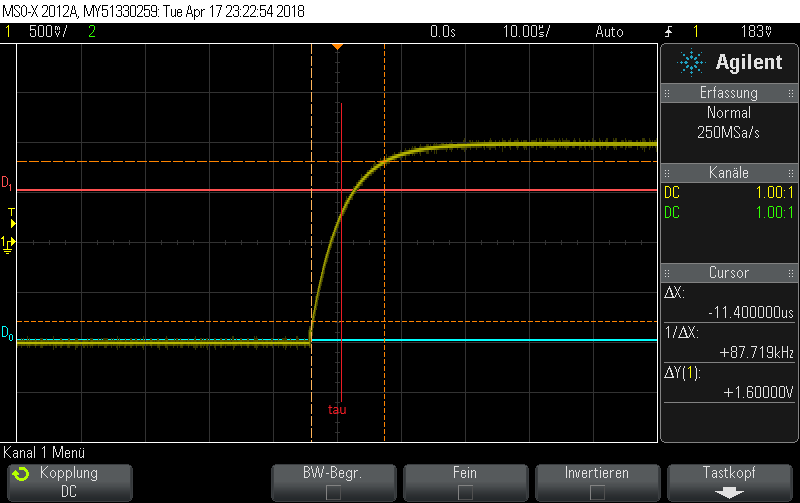
\includegraphics[width=0.7\textwidth]{c_manuell}
    \label{fig:c_man}
    \end{figure}
    Es soll die Kapazität eines Kondensators bestimmt werden. Wir haben dafür das Verhalten mit einem Oszilloskop betrachtet. Der Kondensator wurde an die Rechteckspannung eines Funktionsgenerators mit der einer Frequenz von 1\si{k\Hz} angeschlossen. Die Amplitude lag bei 1\si{V} und die Ausgangslast wurde auf 50\si{\ohm} eingestellt. Im folgenden wurde die Anstiegszeit(Risetime) gemessen und daraus die Kapazität berechnet.\\
    Eine Messung mittels Cursor (Abbildung \ref{fig:c_man}) ergibt eine Risetime von $\Delta t=11,4\si{\micro s}$. Die Zeitkonstante beträgt also $\tau = \frac{\Delta t}{2,2} = 5,18\si{\micro s}$. Die Kapazität berechnet sich durch $C=\frac{\tau}{R}=\frac{5,18\si{\micro s}}{50\si{\ohm}}=103,6\si{n F}$. \\
    Wenn die Risetime mit der Measure Funktion des Oszilloskops gemessen wird, erhält man eine Kapazität von $91\si{n F}$.\\
    Eine direkte Messung der Kapazität mit dem Multimeter ergibt einen Wert von $98\si{n F}$.
    Die Abweichungen lassen sich im ersten Fall mit der Ungenauigkeit beim Ablesen vom Bildschirm erklären. Die eingebaute Messfunktion des Oszilloskop hat leichte Probleme mit kleinen Störungen auf dem Signal und springt deshalb etwas.
    
    \subsection{Tiefpass}
    \paragraph{1. Grenzfrequenz}
    \begin{figure}
    \caption{Grenzfrequenz des Tiefpass}
    \centering
    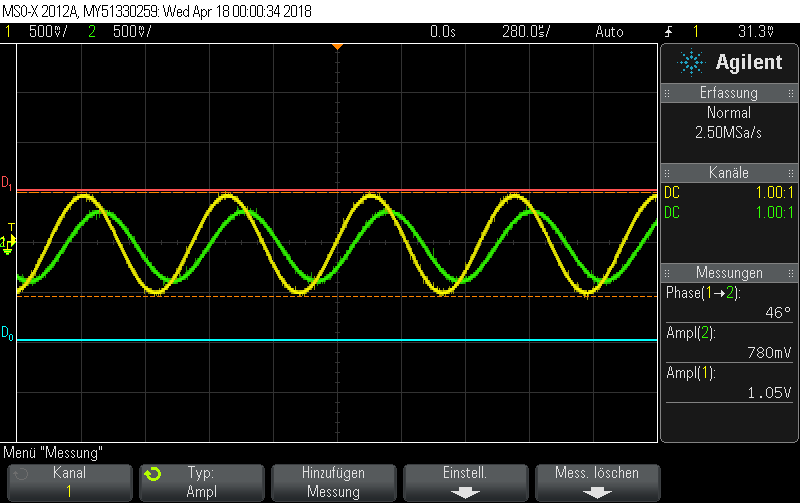
\includegraphics[width=0.7\textwidth]{3db}
    \label{fig:3db}
    \end{figure}
    Bei frequenzabhängigen Schaltungen die verstärken oder abschwächen, berechnet man i.A. eine sogenannte Grenzfrequenz. Die Grenzfrequenz definiert die Frequenz, bei dem das Übertragungsverhältnis des Filters $\frac{1}{\sqrt{2}}$ beziehungsweise $3\si{dB}$ beträgt. Die Phasenverschiebung beträgt bei einem System erster Ordnung dann genau \ $\frac{\pi}{4}$. Die $3\si{dB}$ Grenzfrequenz berechnet sich durch $f_c=\frac{1}{2 \pi R C} = \frac{1}{2 \pi \cdot 1\si{k\ohm} \cdot 100\si{n F}} = 1591,5\si{Hz}$. Bei der Grenzfrequenz beträgt die Dämpfung etwa $0,7$ (Abbildung \ref{fig:3db}).
    
    \paragraph{2.Phasenverschiebung}
    \begin{figure}
    \caption{Messung der Phasenverschiebung}
    \centering
    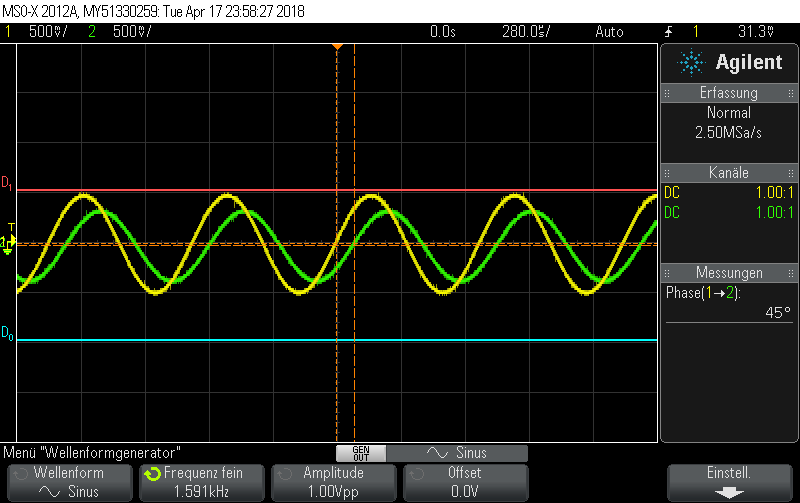
\includegraphics[width=0.7\textwidth]{45deg}
    \label{fig:45deg}
    \end{figure}
    Bei der Grenzfrequenz beträgt die Phasenverschiebung $45$ Grad. Dies wird durch eine Messung (Abbildung \ref{fig:45deg}) belegt.
    
    \subsection{Messung mit Tastkopf}
    \paragraph{1. Richtige Kalibration}
    Der Tastkopf des Oszilloskopes hat im Gegensatz zum einfachen Messkabel einen Einganswiderstand und eine Einganskapazität eingebaut. Zusammen mit den Eingansimpedanzen des Oszilloskopes bilden Sie einen Spannungsteiler. Teilungs- und somit auch Messfehler entstehen, wenn die Zeitkonstanten der Impedanzen von Oszilloskop und Tastkopf nicht gleich sind. Mit Hilfe der Eichspannung ist der Fehler aber leicht erkennen und lässt sich mit der Stellschraube am Tastkopf beheben.
    Ist der Tastkopf mit der Stellschraube richtig kalibriert, wird die Rechteckspannung wie in Abbildung \ref{fig:spitzefixed} richtig dargestellt.
    \begin{figure}
    \caption{Kalibrierter Tastkopf}
    \centering
    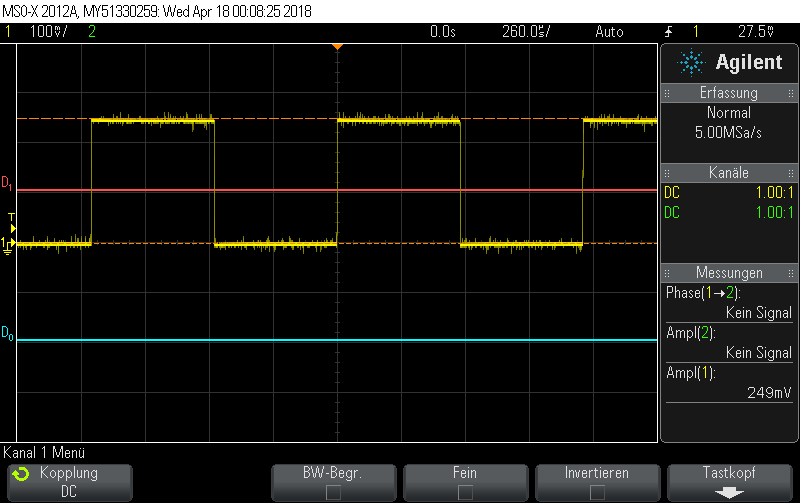
\includegraphics[width=0.7\textwidth]{spitzefixed}
    \label{fig:spitzefixed}
    \end{figure}
    
    \paragraph{2. Dämpfung}
    In Abbildung \ref{fig:spitze1} ist die Abgleichkapazität nicht korrekt, das Signal wird zu sehr gedämpft. Dies bewirkt ein zu langsames Ansteigen des Spannungsverlaufes, sodass das Rechtecksignal nicht präzise dargestellt wird.
    \begin{figure}
    \caption{Dämpfung}
    \centering
    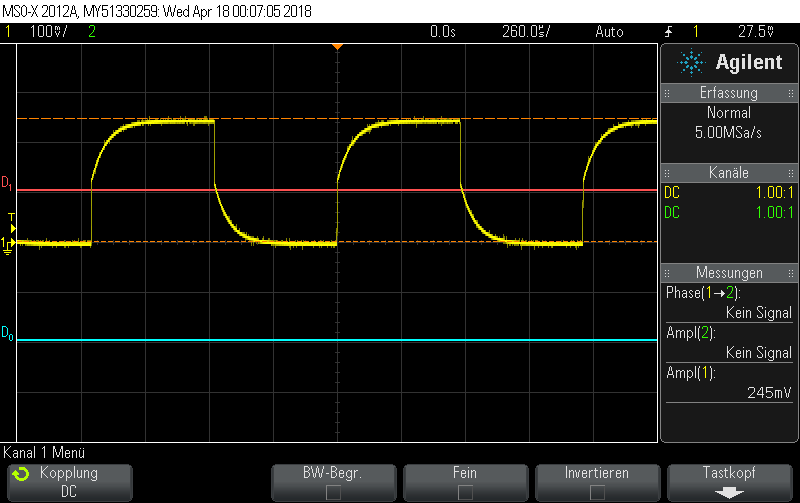
\includegraphics[width=0.7\textwidth]{spitze1}
    \label{fig:spitze1}
    \end{figure}
    
    \paragraph{3. Überschwingen}
    In Abbildung \ref{fig:spitze2} sieht man ein Überschwingen des Signals. Dabei steigt die Spannung an den Flanken zunächst auf einen zu hohen Wert an und nähert sich erst dann der eigentlichen Rechteckschwingung.
    \begin{figure}
    \caption{Überschwingen}
    \centering
    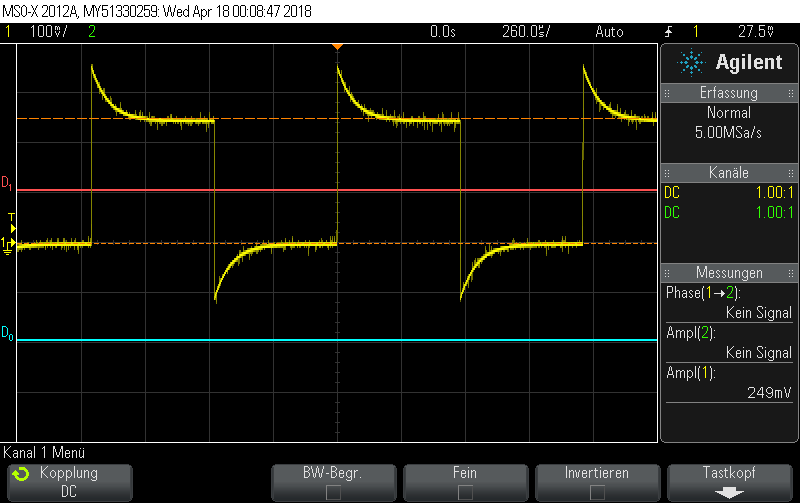
\includegraphics[width=0.7\textwidth]{spitze2}
    \label{fig:spitze2}
    \end{figure}

\end{document}